% $Id: intro.tex,v 1.1.1.1 2007/10/03 22:28:18 hridesh Exp $

\section{Motivation}
Generator functions can generate a function that behaves like an iterator. They allow programmers to make an iterator in a fast, easy and clean way without too much memory cost. To illustrate this, let us consider a simple Python example of building a list and return it\cite{generators}.
%
\begin{figure}[H]
	\centering
	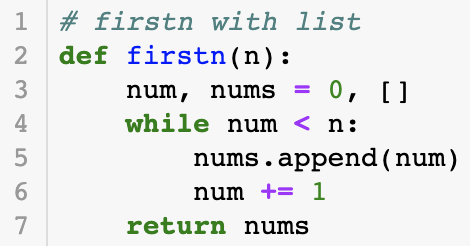
\includegraphics[width=0.4\textwidth]{figures/fstn}
	\caption{Firstn with List}
\end{figure}
%
In figure 1, the function firstn return a full list with length n in memory. If n is really big number and each integer keeps 10 megabyte in memory, then we need to cost a lot of memory to extend our RAM.
%
\begin{figure}[H]
	\centering
	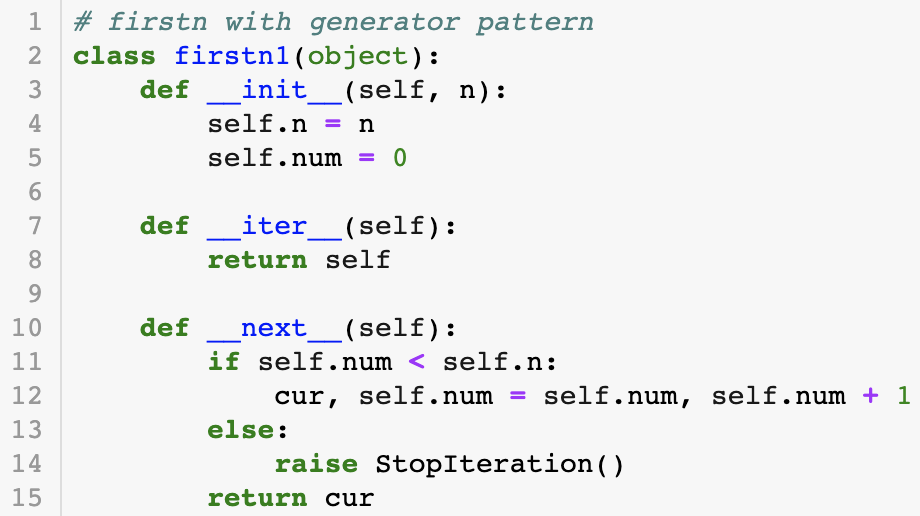
\includegraphics[width=0.75\textwidth]{figures/fstn1}
	\caption{Firstn with List}
\end{figure}
%
To save memory space, we can implement the firstn1 as an object with generator pattern, fig 2. Class firstn1 is iterable and it will perform as we expect. However, we need to write a bunch lines of code to implement it and the logic is expressed in a convoluted way.

%
\begin{figure}[H]
	\centering
	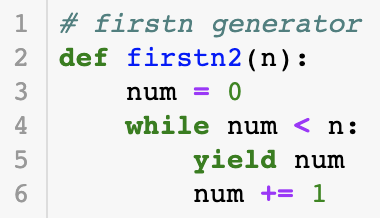
\includegraphics[width=0.4\textwidth]{figures/fstn2}
	\caption{Firstn Generator}
\end{figure}
%

Python provides generator feature in each functions. In the figure 3, the keyword yield indicates that the function firstn2 is a generator that yields items in the iteration instead of returning a list. Compare the actually object sizes in these approaches with the same input 10k. The figure 4 shows that the generator has a huge advantage not only in memory efficiency but also in clear and natural logic. 

%
\begin{figure}[H]
	\centering
	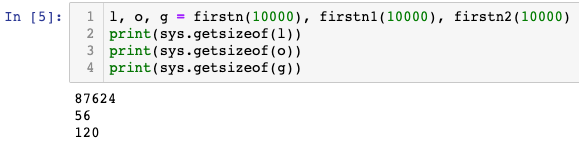
\includegraphics[width=0.75\textwidth]{figures/memsize}
	\caption{Memory Sizes}
\end{figure}
%